\chapter{Methods}
\label{chapter2}

%Everything that comes under the `Methods' criterion in the mark scheme should be described in one, or possibly more than one, chapter(s).

\section{Software Design}

With the necessary background research performed, the next step was to design the architecture of the online learning resource.

\subsection{JupyterLab}

JupyterLab is an interactive computing platform developed by Project Jupyter \cite{jupyter}. It allows users to run code inside their browsers, as well as displaying Markdown and LaTeX. Markdown is a simple language for formatting text. It includes things like headings, bullet points, tables, images etc. It is used widely in documentation, readme files and other educational coding resources. It is incredibly lightweight and easy to write, and it's philosophy is about putting readability first \cite{markdown}. LaTeX is another so called ``mark-up'' language widely used in academic writing. It can be used to construct professional looking documents, and gives the user a massive amount of control in their construction. It also has an extensive set of mathematical symbols, and environments, making it one of the best tools for writing mathematics on a computer. JupyterLab uses a JavaScript library called MathJax \cite{mathjax} to implement the mathematical functionality of LaTeX.

The interface of JupyterLab can be seen in Figure \ref{fig:jupyter-lab}, the main section on the right is where code and markdown is displayed, while the left shows other options. In this figure, it is showing the file tree, although this can also show kernels currently in use, a structured view of the notebook currently open and any extensions.

\begin{figure}[h]
\centering
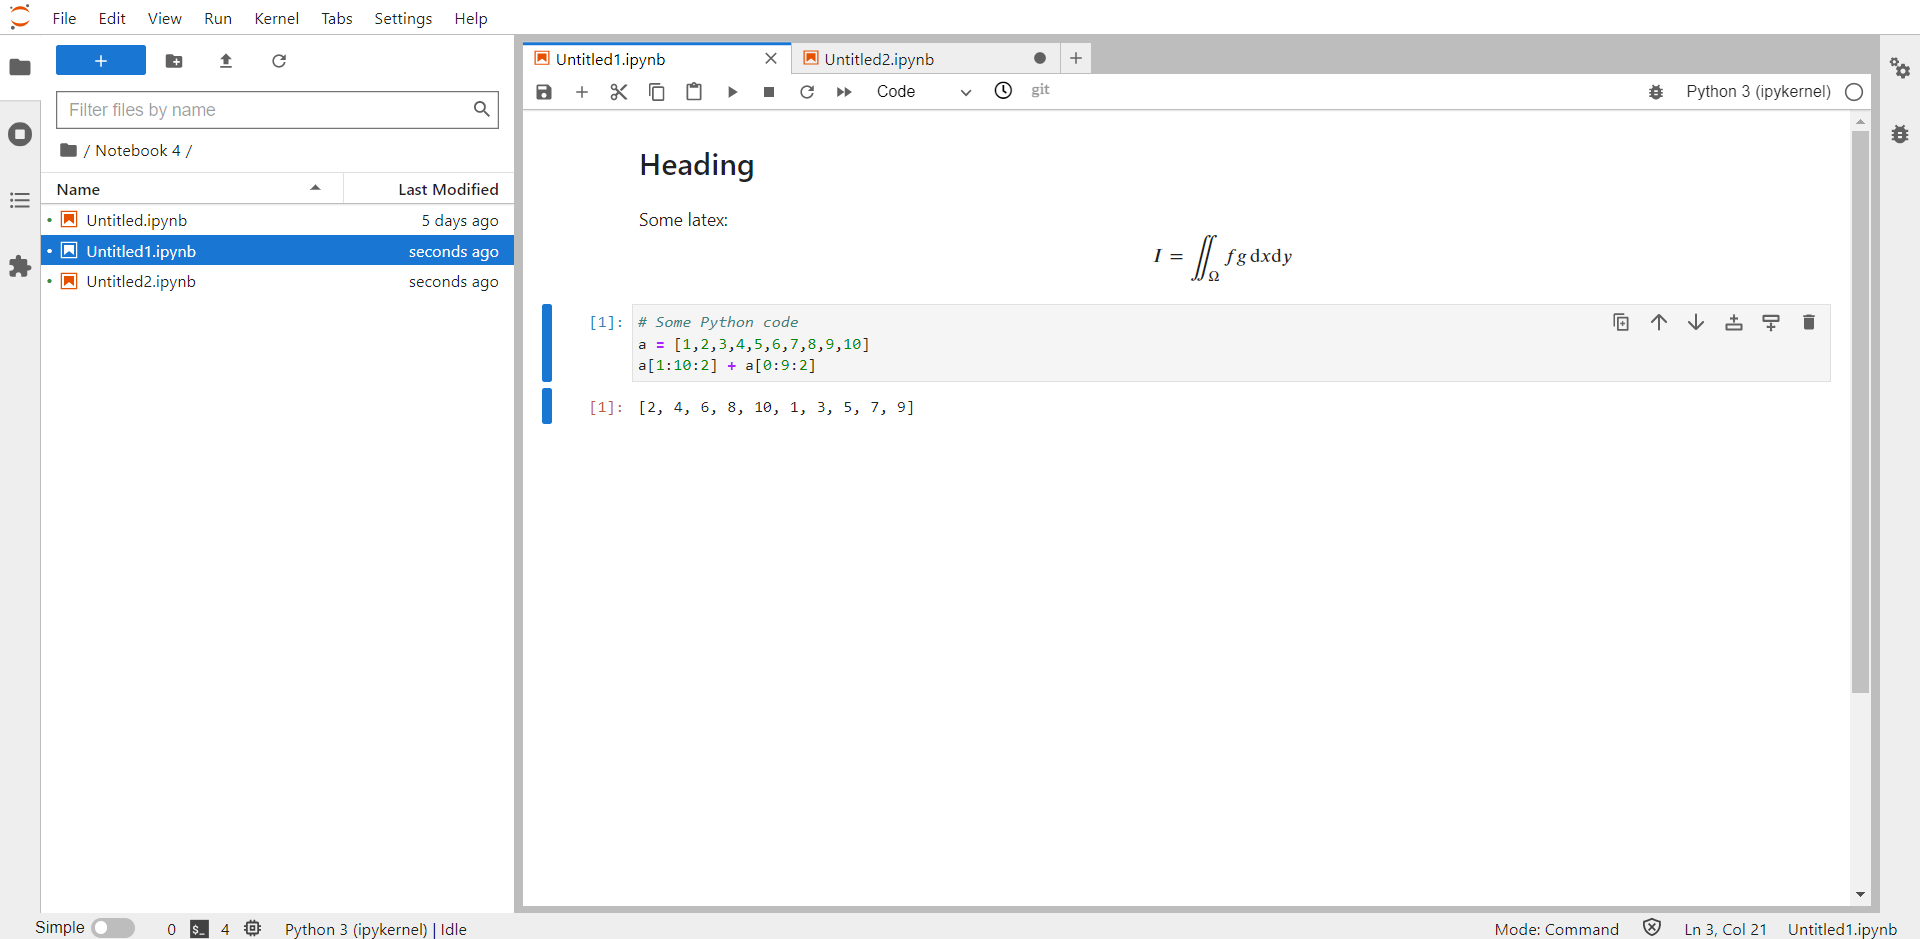
\includegraphics[scale=0.4]{jupyterLab}
\caption{The JupyterLab Interface} \label{fig:jupyter-lab}
\end{figure}

Jupyter is an excellent way of running code for instructional or demonstrative purposes. The LaTeX allows for precise mathematical descriptions, while Markdown keeps everything readable and clean. It is also very quick to write in. Jupyter supports most modern languages by allowing the user to specify a kernel, although the main languages that are supported are Julia, Python and R (Which are the origins of the name Jupyter). In this context, a kernel is the computational engine used to run code within the notebook, of which there are many official versions and community-maintained versions.

\subsection{Python}

The Finite Element library used is called FEniCSx, which was introduced in Section \ref{subsection:overviewOfTools}. The justification behind using this particular platform, is that it provides a good compromise between versatility and complexity. FEniCSx is very versatile because has a lot of features, meaning PDEs arising in any scientific discipline can be solved. It is also easier to pick up than something like FreeFEM++, since it is based solely on Python and there are some good already tutorials already created. In FEniCSx, the most basic PDE instances can be defined, solved and visualised in around fifty lines.

One of the downsides of using FEniCSx is that it has a lot of dependencies. The guide to installing all the source packages can be seen \href{https://docs.fenicsproject.org/dolfinx/main/python/installation.html#source}{here}. At least eleven separate libraries are required for the C++ core, after which one can install the Python interface. Needless to say, this is a time consuming and complicated process. It can be streamlined greatly by instead using Docker.

\subsection{Docker}

Docker is a virtualisation software that allows users to run virtual machines at an operating system level. Each virtual machine is called a container, which is designated its own an area of memory. When creating a docker container, one must specify its contents. This is done by creating an image, a kind of template that containers copy from. Images contain a set of instructions that create directories, download and install programs, and generally set up a container for use. Docker containers are essentially separate, independent environments in which one can work. The point of having these separate environments is to allow for the development of independent software features. As well as it's use for software development, it can also be used to run complicated dependencies. An organisation, such as the Fenics Group, might host a Docker image from which any user can pull. Once the user has the Docker image locally, they are able to create their own Docker containers and work with the organisation's software. The FEniCSx group has such an image! It can be found on the DOLFINx \href{https://github.com/FEniCS/dolfinx#docker-images}{Github page}. 

However, while these docker images are excellent and contain the whole of FEniCSx and more, they don't contain everything necessary for our learning resources. For instance the plotting library Matplotlib is not included in the main Docker image. Also certain timing and meshing libraries are not built in. It is possible to create a Docker image using a DockerFile. In said file, one can pull from an existing image, which is exactly what would be needed in our case. However, the simpler option here was to use a pre-made docker image hosted by Dokken for use with his FEniCSx Tutorial \cite{dokken-docker}.

\subsection{Method of Delivery}

Having created the chosen development environment, a docker container inheriting from Dokken's image, the next logical thought was how to allow users to access the notebooks. One of the main features of a notebook that makes it appealing is the interactive nature of the blocks. User's can run code examples to see dynamically changing outputs. They can alter the author's code in any way they like, or use the dependencies to solve their own problems. As such, the interactive aspect needed to be kept, instead of converting the notebook files to static PDFs. The first method attempted, was to use a service called Binder \cite{binder}. Binder is a service that hosts Jupyter notebooks in an executable environment. This means anyone, anywhere can access the notebooks without setting up any dependencies. They only have to follow a link. Sounds like the perfect solution!

\begin{figure}[h]
\centering
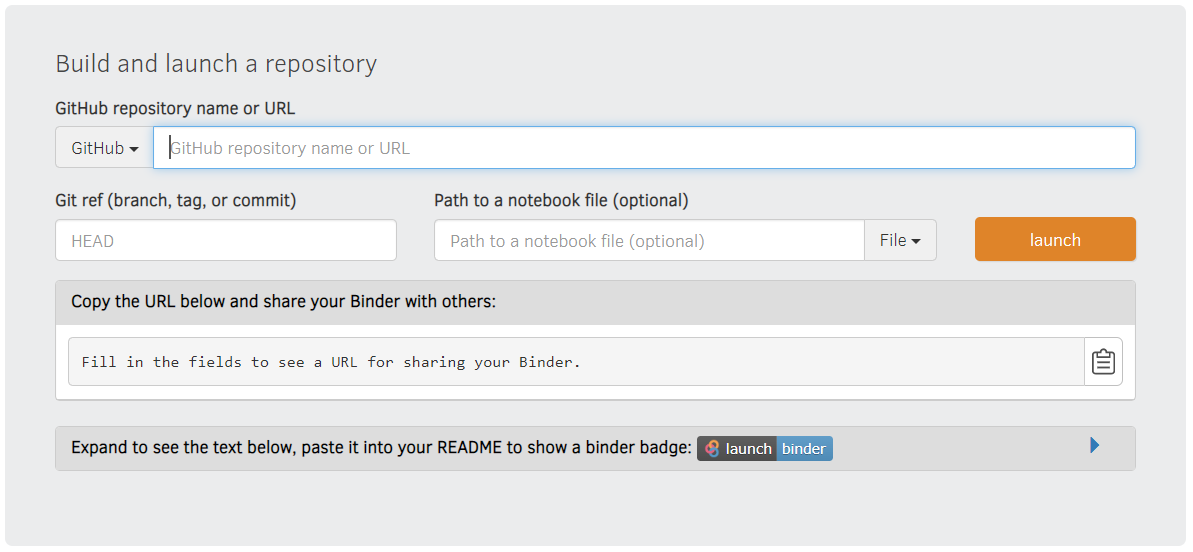
\includegraphics[scale=0.5]{binder}
\caption{Hosting a Jupyter Notebook with Binder} \label{fig:binder}
\end{figure}

All Binder needs to host a notebook is a link to the repository containing said notebooks, plus a few launch options. It's incredibly simple and would work excellently if it wasn't for one problem. The notebook's dependencies can normally be specified by adding a \texttt{requirements.txt} file listing the Python/Julia/R libraries needed and their versions. However, since we have many libraries that are actually built from C++, and require more care to install, this approach will not work. Instead a DockerFile must be provided. This makes sense, because Binder actually uses a Docker container themselves to host the notebooks being run. However, despite the feature being implemented by Binder, they actually discourage users from using it. They consider it an ``advanced use case'' and, crucially, ``cannot guarantee that the DockerFile will work'' \cite{binder-dockerfile-guide}.

Unfortunately, this was indeed the case upon integrating Dokken's DockerFile into the repository used to host the notebooks. Commits \href{https://github.com/Crypto84/FEMLearningResources/commit/de7cec4592aa68bc6e625533d709ff799cfe6452}{de7cec4} through to \href{https://github.com/Crypto84/FEMLearningResources/commit/53e565f6008c000b9800c41ae86256a9d95364e4}{53e565f} were all attempts to get Binder working. It was all based off of Dokken's file, which already worked with Binder in his repository, but when the exact same files were in mine, it didn't work. This was a blow, but in the interest of time, the decision was made to not go with Binder and instead get users to run the notebooks themselves.

Getting users to run the notebooks themselves required them to install Docker on their own machines and create a container themselves. The installation of Docker can be fairly involved to someone who doesn't know the process, since it requires a separate virtualisation software at an OS-level. Linux based operating systems come with native virtualisation, but Windows does not. Therefore, one of the best ways to run docker on Windows is to install Linux on Windows and then perform the containerisation inside of Linux (inside of Windows). Figure \ref{fig:virtualisation} illustrates the hierarchy.

\begin{figure}[h]
\centering
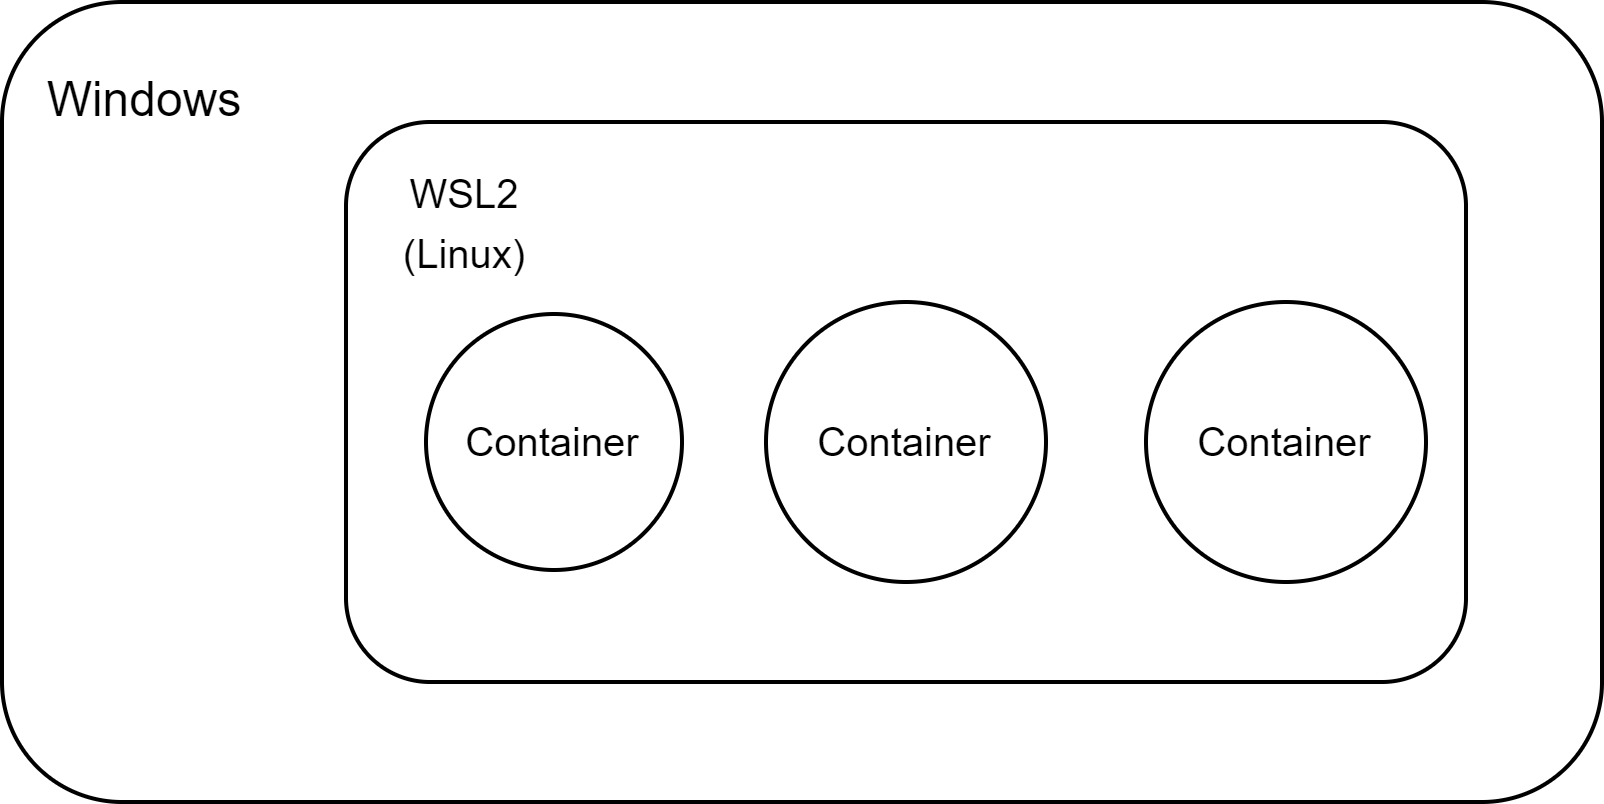
\includegraphics[scale=0.25]{virtualisation}
\caption{Virtualisation Hierarchy} \label{fig:virtualisation}
\end{figure}

The process of installing WSL2 (Windows Subsystem for Linux) is not too complicated, although a guide is certainly required in order to explain the process, and also how to create the container itself. Therefore, since this seemed to be the only option, a guide was created and uploaded to the repository for users convenience. The resulting PDF can be found \href{https://github.com/Crypto84/FEMLearningResources/blob/main/setupGuide.pdf}{here} and describes multiple options depending on the user's system, with the goal being to allow as many students to access the material as possible.

% https://computational-acoustics.gitlab.io/website/posts/30-intro-to-fenics-part-1/ Pros and cons of FENICSx


\section{Content Design}

% Talk about the general design of the solution. What an ideal user experience would look like, and how the experience would flow.

% Accessibility choices

\subsection{User Experience}

A flow diagram of the user experience in the resource's current form is shown in Figure \ref{fig:user-experience}.

\begin{figure}[h]
\centering
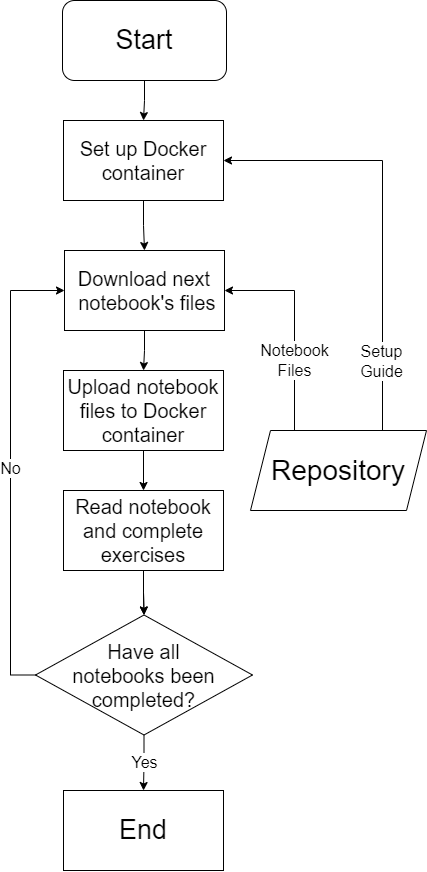
\includegraphics[scale=0.25]{user_experience.drawio}
\caption{Flow Diagram of User Experience} \label{fig:user-experience}
\end{figure}

The user will begin by accessing the repository containing all the notebook files, called \texttt{FEMLearningResources}. From here, they must download and complete the setup guide to install Docker and create their Docker container. Once this is done they will have everything they need to proceed with running and viewing the notebooks in an interactive setting. Next, the user downloads the files for the notebook they are want to read. This needs to be unzipped and then should be uploaded to the Docker container. Jupyter has functionality for uploading documents, so this can be used. Finally, the user can read the notebook, run code blocks and complete exercises.

While this experience is a little more involved than the Binder approach, it does teach students how to use Docker, a very widely used tool in software development. However, it means that the barrier to entry is higher than it needs to be which is unfortunate.

\subsection{Content Plan}

%** Talk about content plan, why I structured it the way I did and why I chose the content I did, always referring back to relevant research. Motivate the need for a mathematical understanding of the problem and it's solution instead of simply solving using packages you don't understand. This section should talk more about the education and mathematics, and should also touch upon the background of my target audience.** (SEE Section 3.3)

With the learning structure defined, we will now discuss the design of the content plan. The initial goal was to teach students to understand and use the Finite Element Method. The belief during the design phase was that ``understanding'' took precedence over ``using''. This is because if one understands the theory behind a method, implementation is broadly the same over different specific libraries. Furthermore, FEniCSx is a library very closely related to the mathematical description of FEM, so a focus on the mathematics would lead more naturally into this. Another balance that was considered was between simplicity and complexity. Making the content too simple would not meet the goal of the project and would leave students feeling dissatisfied. Making the content too complex by increasing the scope would put pressure on the time constraints of the project, and may lead to students feeling rushed or unsure about certain topics due to the less considered development. This is how to original content plan was developed. It can be seen in Figure \ref{fig:og-content-plan}.

\begin{figure}[H]
\centering
\begin{subfigure}{.5\textwidth}
  \centering
  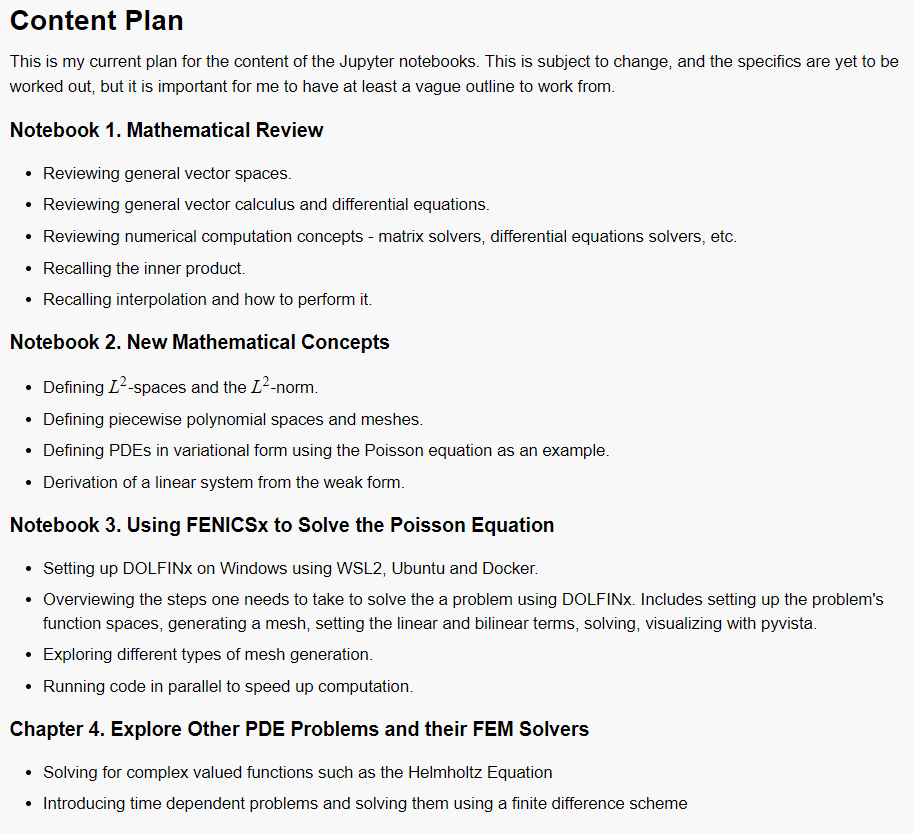
\includegraphics[scale=0.4]{og_content_plan}
  \caption{Original Content Plan} \label{fig:og-content-plan}
\end{subfigure}%
\begin{subfigure}{.5\textwidth}
  \centering
  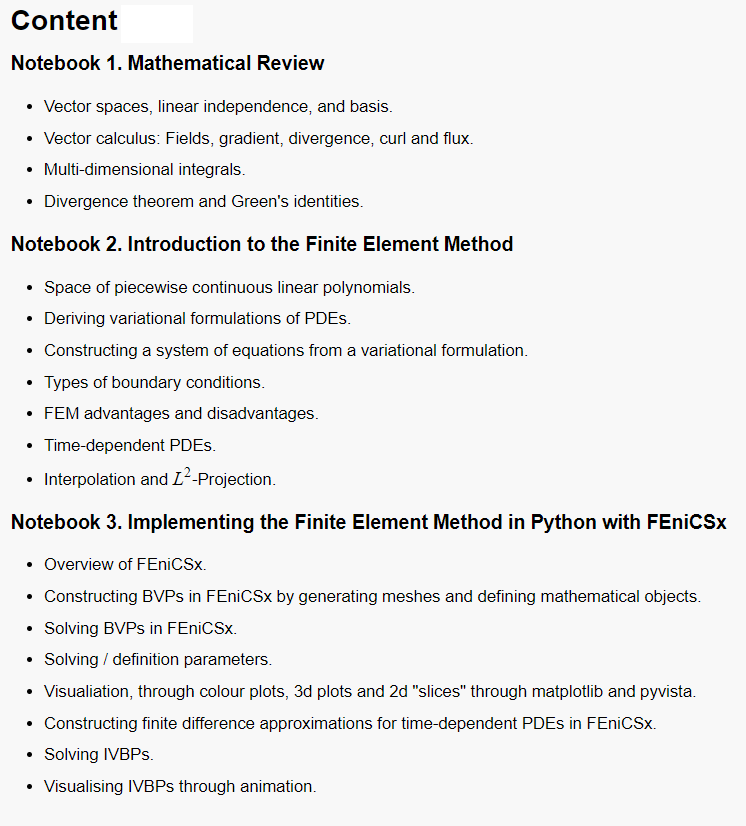
\includegraphics[scale=0.4]{new_content_plan}
  \caption{Updated Content Plan} \label{fig:new-content-plan}
\end{subfigure}
\caption{Change in content between start and end of the project}
\label{fig:test}
\end{figure}

The content originally spanned 4 Notebooks, each of increasing complexity and interest to the reader. The notebooks were to begin with a general mathematical review, preparing the reader for the new mathematics that was to follow. The reader was assumed to have a mathematical knowledge of a second or third year mathematics undergraduate student and basic knowledge of coding. This influenced the pace at which new material could be introduced as well as the topics that need to be included in the review. Topics like vector calculus, linear algebra and differential equations should be familiar to them, so could be covered in a less detailed way than the FEM content. It felt important to ease the readers in with a refresher, because rushing into new advanced mathematics could lead to confusion. They may have studied the concepts a while ago, so a reminder was important. As such, an entire notebook was devoted to revising these subjects.

Next was the first notebook of new content. The content can be seen in the figure, but it included all of the basic mathematical definitions and procedures for understanding the Finite Element Method. The third notebook was intended to give the readers a chance to get to grips with the implementation of the method. Originally, this is the point the setup guide was needed. The first two notebooks did not have interactive elements and were planned to be static resources. It was decided at a later point that even non-interactive parts of the resource would be created using the notebook format.

Finally, the fourth notebook was planned to give more complicated examples, such as the Helmholtz Equation, a PDE defined for complex-valued variables. Also the modelling of time-dependent systems was to be explored. This was left partially empty due to the idea that additional sections would be added later.

When development began, the content plan had to change. This was because a greater understanding of FEM had been obtained and certain aspects were deemed unnecessary to the goals of the project. Furthermore, a more refined idea of scope was developed, leading to the eventual cut of certain sections. This led to the refinement of four notebooks, to three. The revised syllabus can be seen in Figure \ref{fig:new-content-plan}. A brief explanation of changes is listed below.

\begin{itemize}
    \item Differential equations were removed from the review since enough knowledge could be gained from the vector calculus definitions to make this irrelevant.
    \item A precise description of inner products was removed since it wasn't all that necessary for understanding the function spaces involved.
    \item Emphasis was taken away from the $L^2$ spaces, they would still be mentioned, but it was not all that important to devote much time to them.
    \item Boundary conditions and FEM advantages and disadvantages were added.
    \item Some content was rearranged to increase flow and motivate future sections, specifically interpolation and time-dependent PDEs.
    \item Certain points were made much more specific.
    \item Descriptions of the parallel computation, different types of mesh generation and complex-valued PDEs were all dropped due to make the scope of the project more realistic.
\end{itemize}

\subsection{Adapting the content}

In order to maintain accuracy and correctness, the specific content of the notebooks had to be derived from well-respected and accurate sources. Notebook 1 spans the broadest spectrum of topics, and as such, was derived from the most sources. Knowledge gained from studying mathematics at university came in useful, but s set of invaluable resources in refreshing my memory was the lecture notes provided by module leaders at the University of Leeds. These modules included the following.

\begin{itemize}
    \item MATH2022 Groups and Vector Spaces
    \item MATH1005 Core Mathematics (Introductory calculus, linear algebra and differential equations)
    \item MATH2365 Vector Calculus
    \item MATH2375 Linear Differential Equations and Transforms
\end{itemize}

They were useful not only for the correctness and accuracy of the mathematical statements, but also for their use in explaining concepts in a natural way. While these made up most of the sources for Notebook 1, Wolfram MathWorld \cite{wolfram-mathworld} also played a part in filling in some of the gaps where alternative or additional explanations were needed.

Notebook 2 was based primarily off Bengzon and Larson's textbook \cite{bengzon-larson-fem}. Inspiration was taken from the structure of the book. The authors decided the first two chapters should explain piecewise polynomial spaces and the finite element method in 1 dimension only. This means the domain being solved over was an interval on the number line. Since there is only one variable to differentiate with respect to, this simple case is an ODE, not a PDE. The simplicity enabled the reader to build upon the base knowledge presented and progression to higher dimensions followed very naturally.

Most of Notebook 3's material was taken from Dokken's tutorial \cite{fenics-tutorial}. His tutorial is one of the only learning resources on FEniCSx available and is by far the most accessible and well-written. Due to this fact and also due to the complexity of the library, a large portion of the code presented in Notebook 3 was written by Dokken. However, the explanations he gives in the tutorial can sometimes be a little shallow, and care has been taken to expand and enlighten. A particularly interesting tangent was on bounding-box trees, a type of data structure that can be used to sort objects in space by the size of their bounding-box. An excellent source for this was this blog post by James from Azure From The Trenches \cite{aabb-tree}

\subsection{Notebook Structure}

The structure of the notebooks was laid out much like a book, with distinct sections and subsections of content separated with exercises. Each notebook was split into two or three sections each tackling a distinct area of study. Notebook 1 contains \textbf{Vector Spaces} and \textbf{Vector Calculus}. Notebook 2 contains \textbf{FEM in 1D}, \textbf{FEM in 2D}, and \textbf{Time Dependent Problems}. Notebook 3 contains \textbf{Introduction to FEniCSx} and \textbf{A Time Dependent Example}. Within these sections, there are a varying number of subsections that break the content up into more manageable topics. These can be seen in Figure \ref{fig:notehereyet}.

Development of the exercises was another important part of the design. Exercises serve to test understanding and cement newly ingested information. They can also be great at challenging possibly incorrect assumptions students may have picked up from the content. After each subsection in a notebook, there were a collection of ``check'' exercises. These ranged from simple calculations, to proving statements in the text, to explanations and sometimes more complicated derivations. For the computing side, exercises were harder to prescribe for each subsection, since an entire section spanned a single example. However, at the end of each section, a chance to apply the methods learned was given through way of practise question. There were even exercises that linked between each other in building a full PDE approximation, which was intended to leave a sense of learner satisfaction in creating their own approximation the whole way through.

\section{Development Methodology}

% GitHub, version control
% Gantt chart
% Agile
% Eventual failure
% Reverting to waterfall

Throughout the development of the project, version control was used to store 